\subsection{Resulting Route}\label{sec:results}
With seed \DCSeed{}, the Divide and Conquer algorithm returns the closed route
\begin{center}
\DCRoute{}
\end{center}
with a total driving distance of \textbf{\DCTotal{} km}. Table~\ref{tab:legs} gives each leg, and
Figure~\ref{fig:route} draws the route on the map.

\begin{table}[H]
\centering
\caption{Legs of the Divide and Conquer route and the recomputed total (km).}\label{tab:legs}
\vspace{4pt}
\footnotesize
\setlength{\tabcolsep}{3.5pt}
% AUTO-GENERATED by code/main.py --export-latex. Do not edit; re-run the export instead.
\begin{tabular}{c l l r r}
\toprule
\textbf{Leg} & \textbf{From} & \textbf{To} & \textbf{km} & \textbf{Cumulative} \\
\midrule
1 & V0 USTP Cagayan de Oro Campus & V1 Limketkai Center & 1.09 & 1.09 \\
2 & V1 Limketkai Center & V7 Port of Cagayan de Oro & 2.32 & 3.41 \\
3 & V7 Port of Cagayan de Oro & V9 Capitol University & 1.79 & 5.20 \\
4 & V9 Capitol University & V2 Centrio Mall & 0.58 & 5.78 \\
5 & V2 Centrio Mall & V3 Pelaez Sports Center & 1.18 & 6.96 \\
6 & V3 Pelaez Sports Center & V4 Museo de Oro (Xavier University) & 1.31 & 8.27 \\
7 & V4 Museo de Oro (Xavier University) & V5 Divisoria Plaza & 0.54 & 8.81 \\
8 & V5 Divisoria Plaza & V6 St. Augustine Metropolitan Cathedral & 0.74 & 9.55 \\
9 & V6 St. Augustine Metropolitan Cathedral & V8 Liceo de Cagayan University & 1.65 & 11.20 \\
10 & V8 Liceo de Cagayan University & V0 USTP Cagayan de Oro Campus & 2.62 & 13.82 \\
\midrule
\multicolumn{3}{r}{\textbf{Total}} & \multicolumn{2}{r}{\textbf{13.82 km}} \\
\bottomrule
\end{tabular}

\end{table}

\begin{figure}[H]
\centering
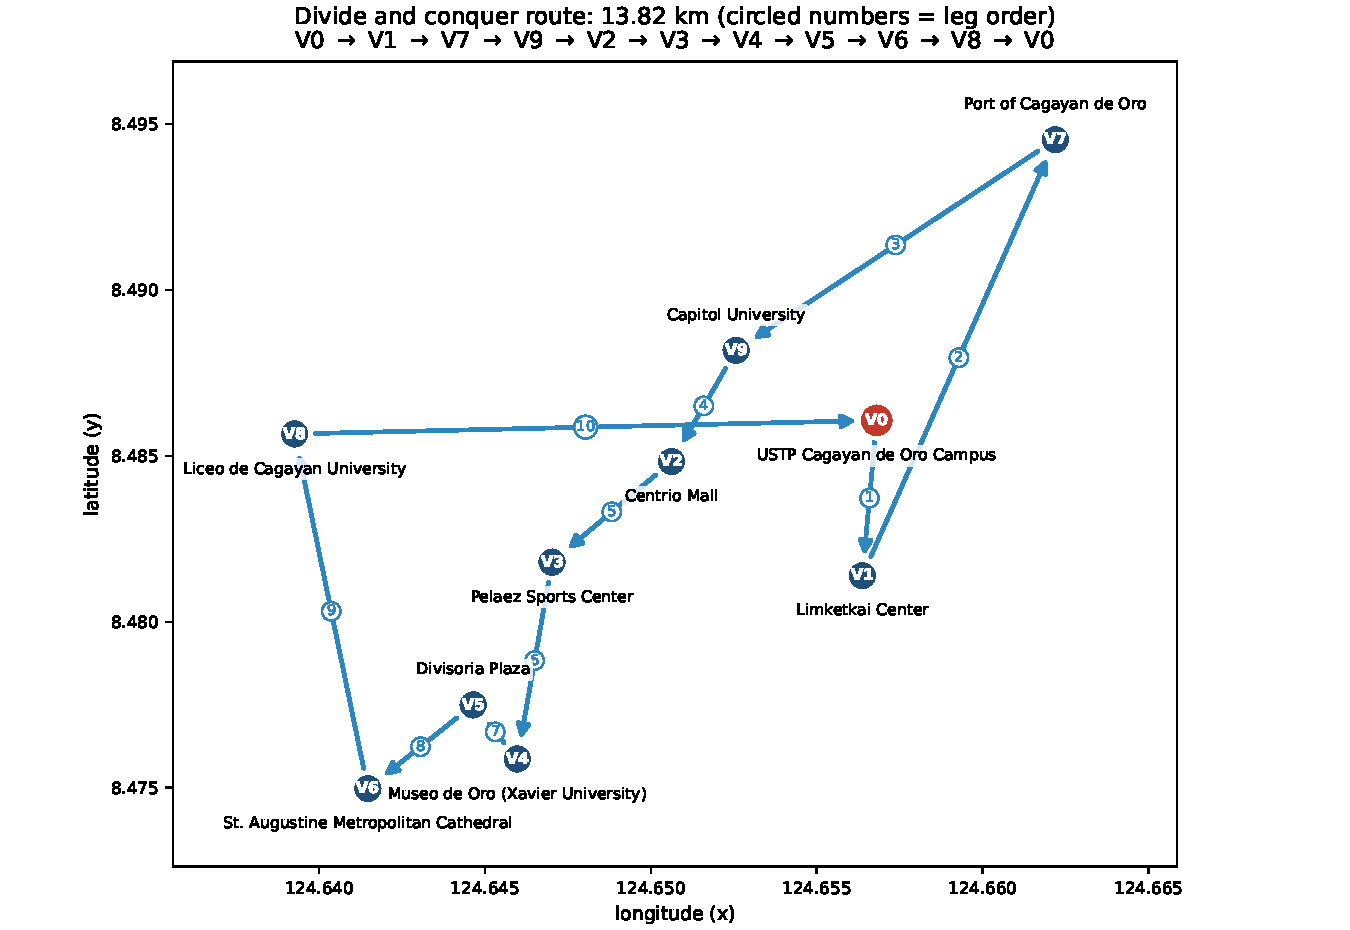
\includegraphics[width=0.85\textwidth]{route.pdf}
\caption{Divide and Conquer route (seed \DCSeed{}). Circled numbers give the order of the legs.}\label{fig:route}
\end{figure}

\paragraph{Interpretation.} The route meets the objective's constraints: the guests leave USTP, visit
each of the nine landmarks exactly once, and return to USTP. It forms one loop: south to Limketkai,
north to the port, then south-west through Capitol University, Centrio, Pelaez, Museo de Oro,
Divisoria and the Cathedral, and finally north-west to Liceo before heading back east to USTP. Because the divide step groups
nearby places, the tight cluster around Divisoria (V4, V5, V6) is visited consecutively using its
shortest edges (0.54 and 0.74~km). The weakest part is the last leg, Liceo (V8) back to USTP
(2.62~km). It was created by the final merge (Table~\ref{tab:trace}), which had to reconnect the two
halves through the shortest bridge V2--V3 and therefore closed the loop with the long edge V8--V0.
This is the ``boundary effect'' limitation of Section~\ref{sec:algorithm} appearing in practice.
